\chapter{Discussion}
Results suggest that our model is suitable for single-objective and multi-objective optimization of generating molecules with target properties, such as ClogP and CMR. This project is an extension of \cite{lee2022mgcvae}, where we used the initial graph matrix to perform an atom-based graph representation system. While \cite{richards2022conditional} proposed a $\beta$-CVAE for \textit{de novo} drug design using SMILES, our project differs by representing molecules with molecular graphs instead of SMILES. This suggests that this project is novel and we could continue our final year project in this direction.

\section{Limitations}
\subsection{Data set} Compared to previous studies in \cite{lee2022mgcvae, richards2022conditional}, our study used a significantly smaller data set of 20,000. In short, \cite{lee2022mgcvae} used a data set of 1,363,452 molecules to train their models while \cite{richards2022conditional} used the ZINC-250k data set with 250,000 random samples from the ZINC database. In addition, we took our data set from the first gun-zipped chunk file provided by the ZINC database for this study. The categorization of ZINC molecules in the database was not considered when selecting the arbitrary chunk file. This could have limited the training of our models. Loosely speaking, we recall that VAE models aim to minimize reconstruction loss to generate molecules similar to the data set. As such, using a larger data set could improve our model performance to generate more diverse drug candidates. We chose 20,000 molecules as the maximum number of molecules due to the lack of GPU RAM in the device used for this project. 

The models generated molecules with 8 types of atoms due to the data set constraints presented in our methods section. This possibly limited our models to generate less sophisticated compounds using more types of atoms. 

\subsection{Challenges} We spent a significant amount of resources during the semester on Generative Flow Networks (GFlowNets) \cite{https://doi.org/10.48550/arxiv.2111.09266}. We initially discussed introducing multi-objective optimization to the GFlowNets. However, we encountered hardware limitations that may require more complex resources. Subsequently, we conducted a study to predict graph properties, where the graph convolutional network and principal neighbourhood aggregation (PNA) models were used to predict graph-based molecular properties \cite{sun2020graph, kong2021end}. This study improved our domain knowledge in graph neural networks, \textit{de novo} drug design, and deep generative models. Subsequently, we combined both ideas of multi-objective optimization with property prediction and conducted research in graph-based VAE models to generate novel compounds. 

\section{Future work}
\subsection{Data set} We aim to increase our data set used to train the models. A more in-depth study should be conducted on the ZINC database to select an appropriate data set. We may consider the use of the National University of Singapore's High Performance Computing (HPC) to meet our computational needs.

\subsection{Models} In this work, we arbitrarily chose $\beta = 2$ and did not experiment with various values of $\beta$. Further research is required to evaluate an appropriate $\beta$ value. We also could explore dynamic $\beta$-VAE suggested in \cite{rydhmer2021dynamic} subjected to conditional information. Similarly, \cite{shao2020controlvae, shao2021controlvae} suggested tuning the VAE using control theory. A possible direction could involve the design of self-tuning control schemes for $\beta$ tuning using neural networks instead of Proportional-Integral controllers for VAE in the context of \textit{de novo} molecular generation \cite{ang2018proposed}. 

In this study, we only used two-layered encoders and decoders in our models as shown in Fig. 4. We used standard AE hidden dimensions of 512 and 256. It is important to note that the VAE framework is similar to dimensionality reduction algorithms or principal component analysis. Hence, the shallow depth of the deep generative VAE models may adversely impact the vectors in the latent space as the dimensions could be prematurely reduced. Therefore, we could improve our results by experimenting with the depth in the layers of our VAE models. 

\subsection{Network training}
We could investigate how the newly proposed gradient descent algorithm impact the results and model training \cite{DBLP:journals/corr/abs-1909-13371}. While we did not conduct a study on the loss curves, training time, and hyperparameters, we noticed that the optimizer increased the training time. Furthermore, Fig. 5 suggests overfitting of our model, which could have affected our model performance. We did not encounter overfitting when using PyTorch's Adam optimizer and scheduler. Further research could be conducted to investigate the training using Adam \textit{gdtuo}.

\subsection{Multi-objective optimization}
ClogP and CMR were chosen as the properties to optimize. In the future, we could evaluate how changing one of CLogP and/or CMR affects QED and SAS. We recall these property terms from the subsection on property optimization in our literature review. In brief, SAS refers to the synthetic accessibility score and QED refers to the quantitative estimate of drug-likeness. Moreover, we could increase the condition vectors to include the optimization of QED and SAS. \cite{lee2022mgcvae} verified their models by redefining the conditioning vectors as follows:
\begin{equation}
    \begin{aligned}
    & C1 = SAS = \{2, 3, 4, 5\}\\
    & C2 = QED  =\{0.5, 0.6, 0.7, 0.8\}. \label{eq}
    \end{aligned}
\end{equation}
 An extension to our work could test the multi-objective optimization of the four molecular properties simultaneously. 

\subsection{Evaluation}
To improve the evaluation matrix, the molecular fingerprints of the generated molecules should have been used to verify that the molecules were similar to the data set. We based our evaluation on validity, novelty, and uniqueness on \cite{https://doi.org/10.48550/arxiv.1705.10843}. This project removed invalid SMILES by converting the generated SMILES into molecules using RDkit and handling the exception error, which removes the invalid SMILES. In terms of novelty, we compared if the SMILES generated were similar to the SMILES in the data set. While it is not incorrect to use this method, the number of novel molecules could have been inflated. For uniqueness, we compared string-wise for duplicate SMILES. The evaluation metrics in this project could be improved by using the molecular fingerprints method and other molecular library similarity tools to evaluate our model.  

We could also investigate if our proposed model could generate more sophisticated molecules than its simpler VAE counterparts. Based on Fig. 7, we hypothesize that more sophisticated molecules could be generated with the $\beta$-CVAE, although no research was conducted in our study. 

\subsection{Gantt chart}
Fig. 8 shows the Gantt chart of our project in AY22/23. It includes the key dates for submission of the deliverables. In the Gantt chart for this interim submission, we exclude the key details for this project the future directions of this project have yet to be discussed.

\begin{figure}[htbp]
    \centerline{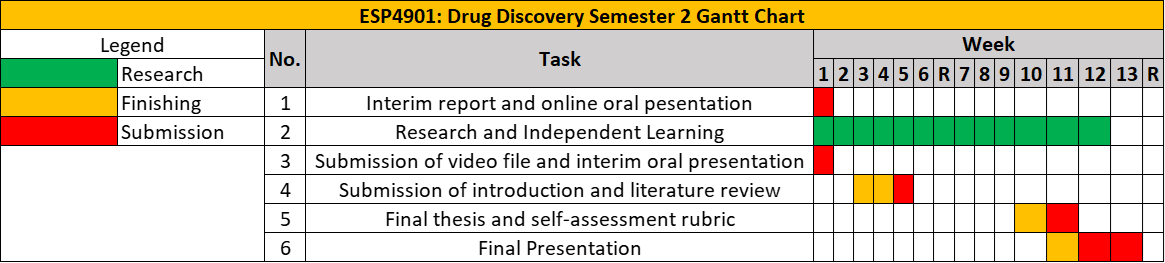
\includegraphics[width=0.5\textwidth]{gantt.png}}
    \caption{Gantt chart for AY22/23 Semester 2.}
    \label{fig}
\end{figure}